% !TEX TS-program = pdflatex
% !TEX encoding = UTF-8 Unicode

\documentclass[fleqn]{article}
\usepackage[utf8]{inputenc} 
\usepackage[left = 2cm, right = 1.5cm, top = 1cm, bottom = 2cm, bindingoffset = 0cm]{geometry} 
\usepackage{import}
\usepackage{Other/Cup}

\title{Introduction to Enumerative Combinatorics \\ Graded assignment 1 \\ V. R. Mozgovoy}

\makeatletter
\newenvironment{sqcases}{%
	\matrix@check\sqcases\env@sqcases
}{%
	\endarray\right.%
}
\def\env@sqcases{%
	\let\@ifnextchar\new@ifnextchar
	\left\lbrack
	\def\arraystretch{1.2}%
	\array{@{}l@{\quad}l@{}}%
}
\makeatother

\begin{document}
	\noindent
	\newpage		
	\section*{Лист 3}
		\subsection*{1}
		\noindent
		Идеальный треугольник состоит из 3 вершин и 3 сторон(геодезических), а следовательно имеет ту же группу симметрий что и граф $K_3$, то есть $D_3$.
		
		\subsection*{2}
		\begin{figure}[h!]
			\begin{minipage}[h]{0.5\linewidth}
				\center{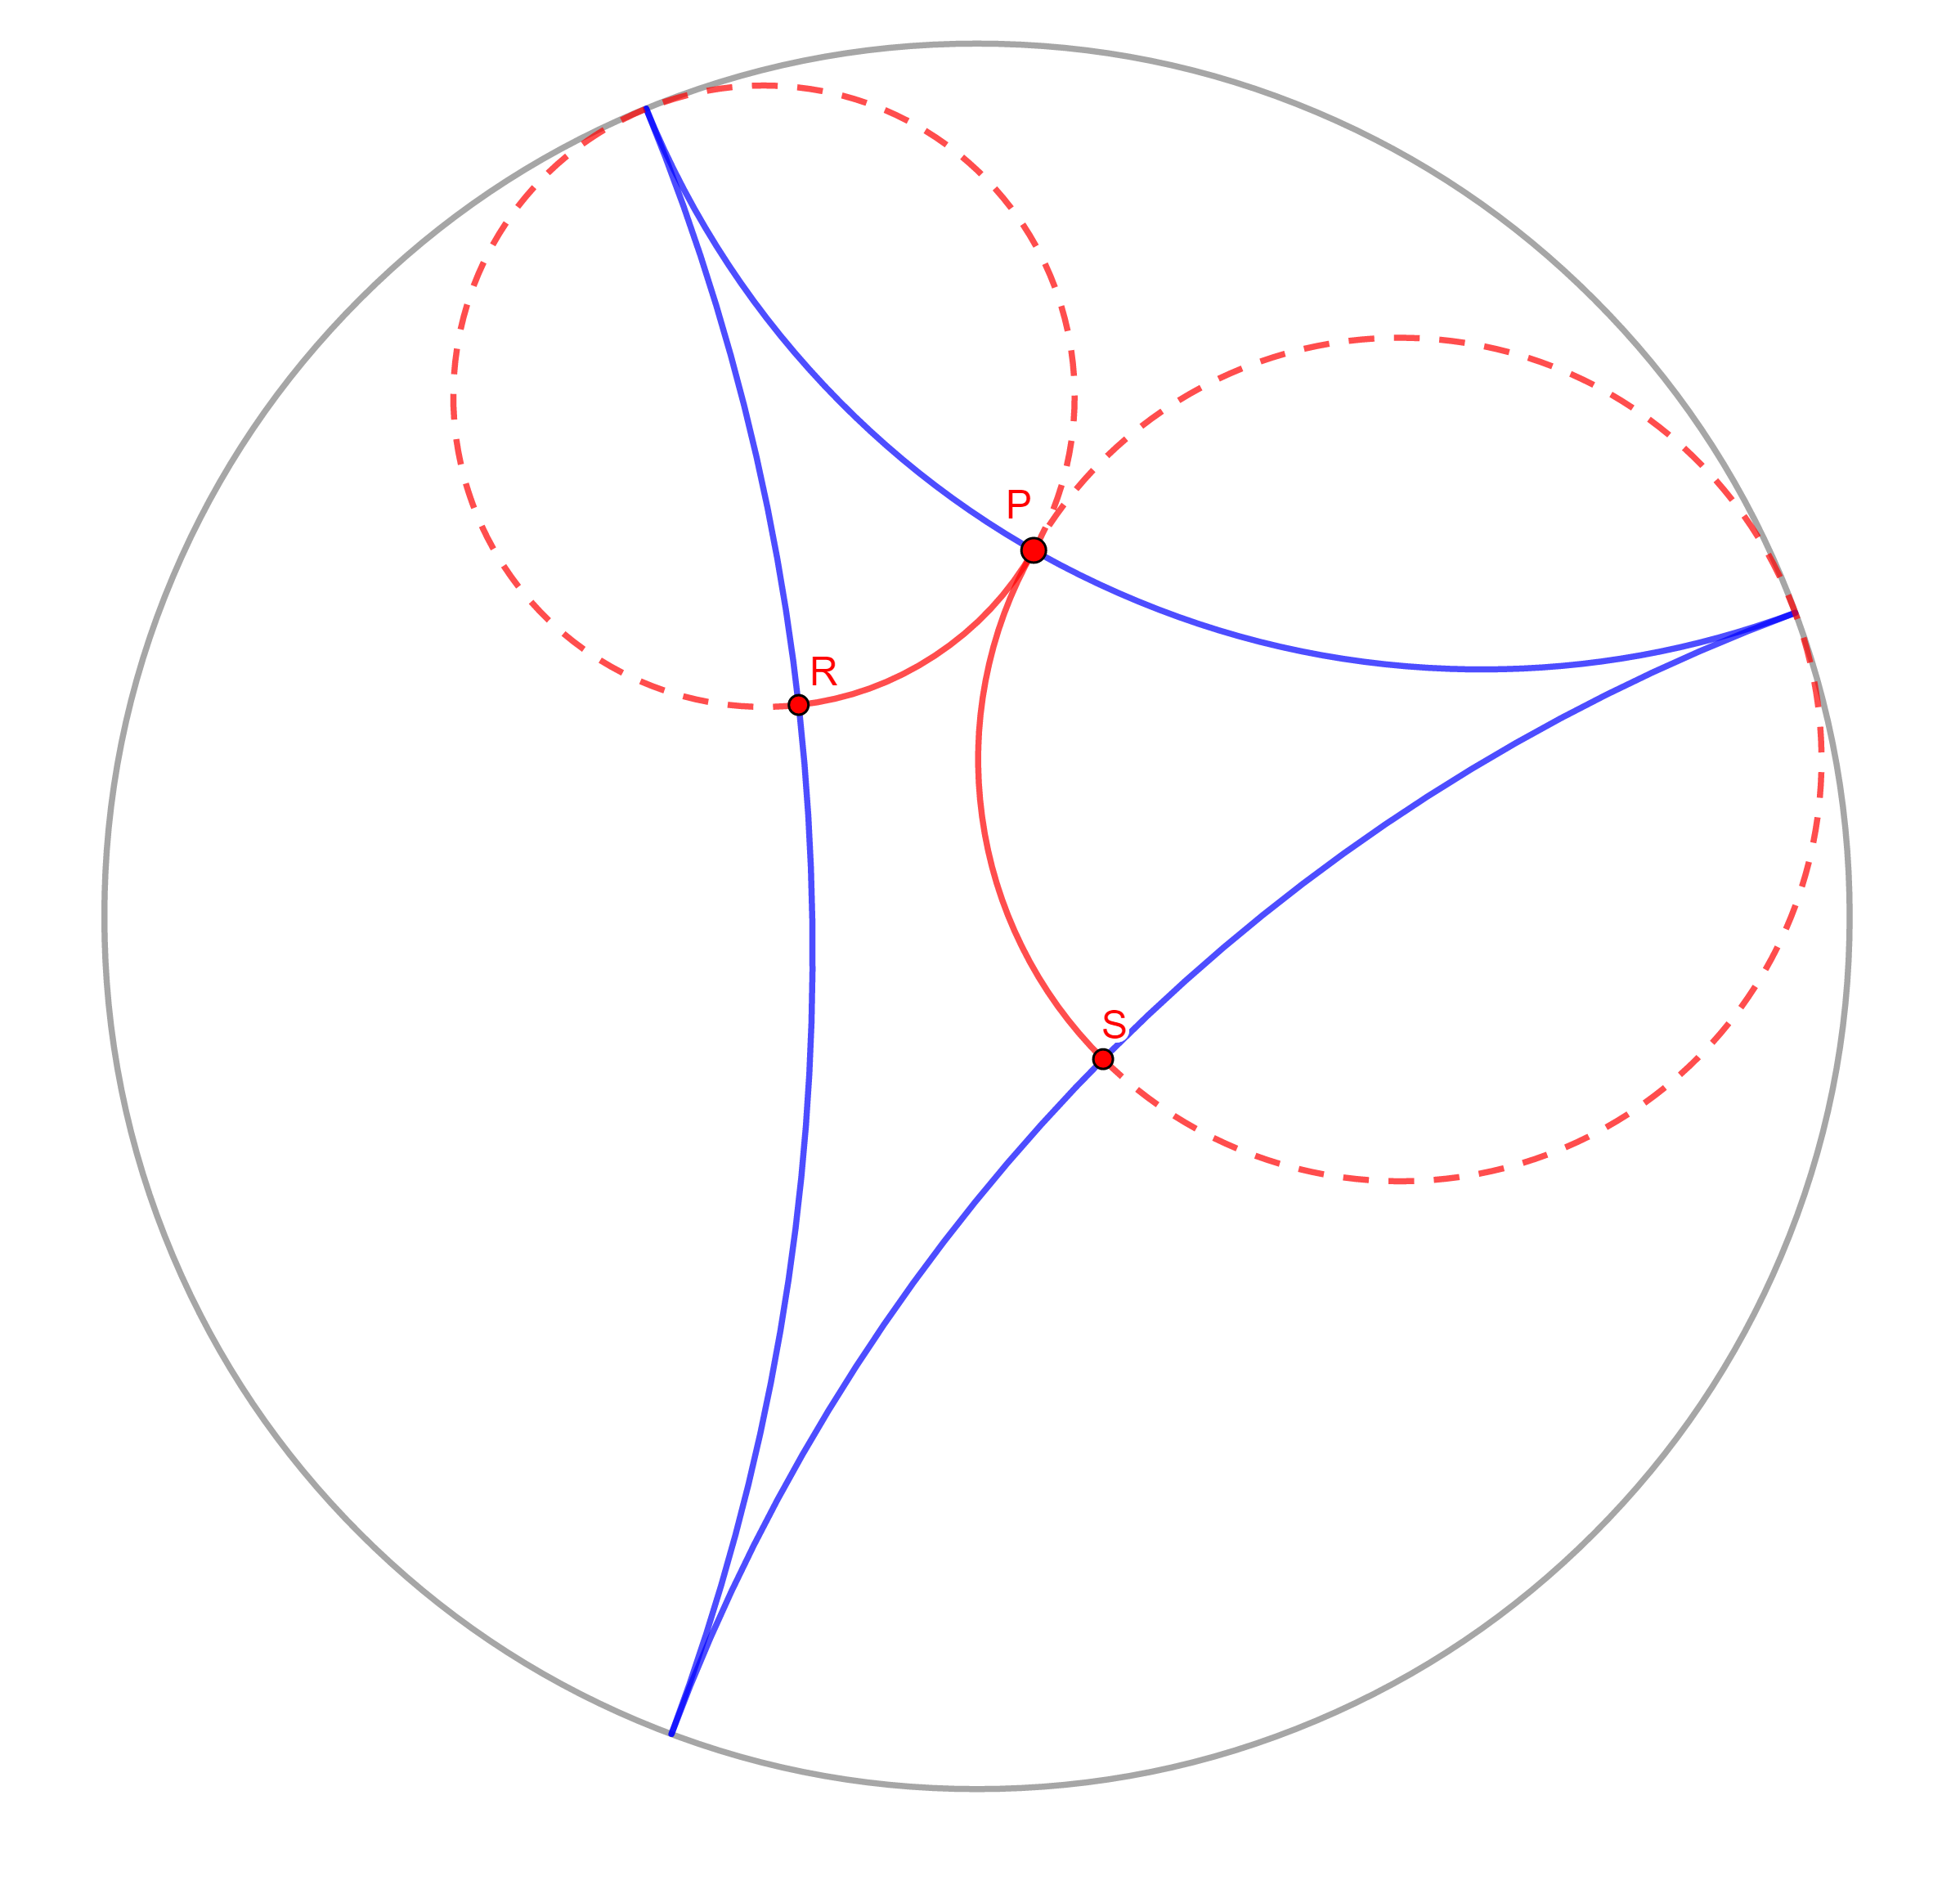
\includegraphics[width=0.7\linewidth]{pic11}}
			\end{minipage}
			\hfill
			\begin{minipage}[h]{0.5\linewidth}
				\center{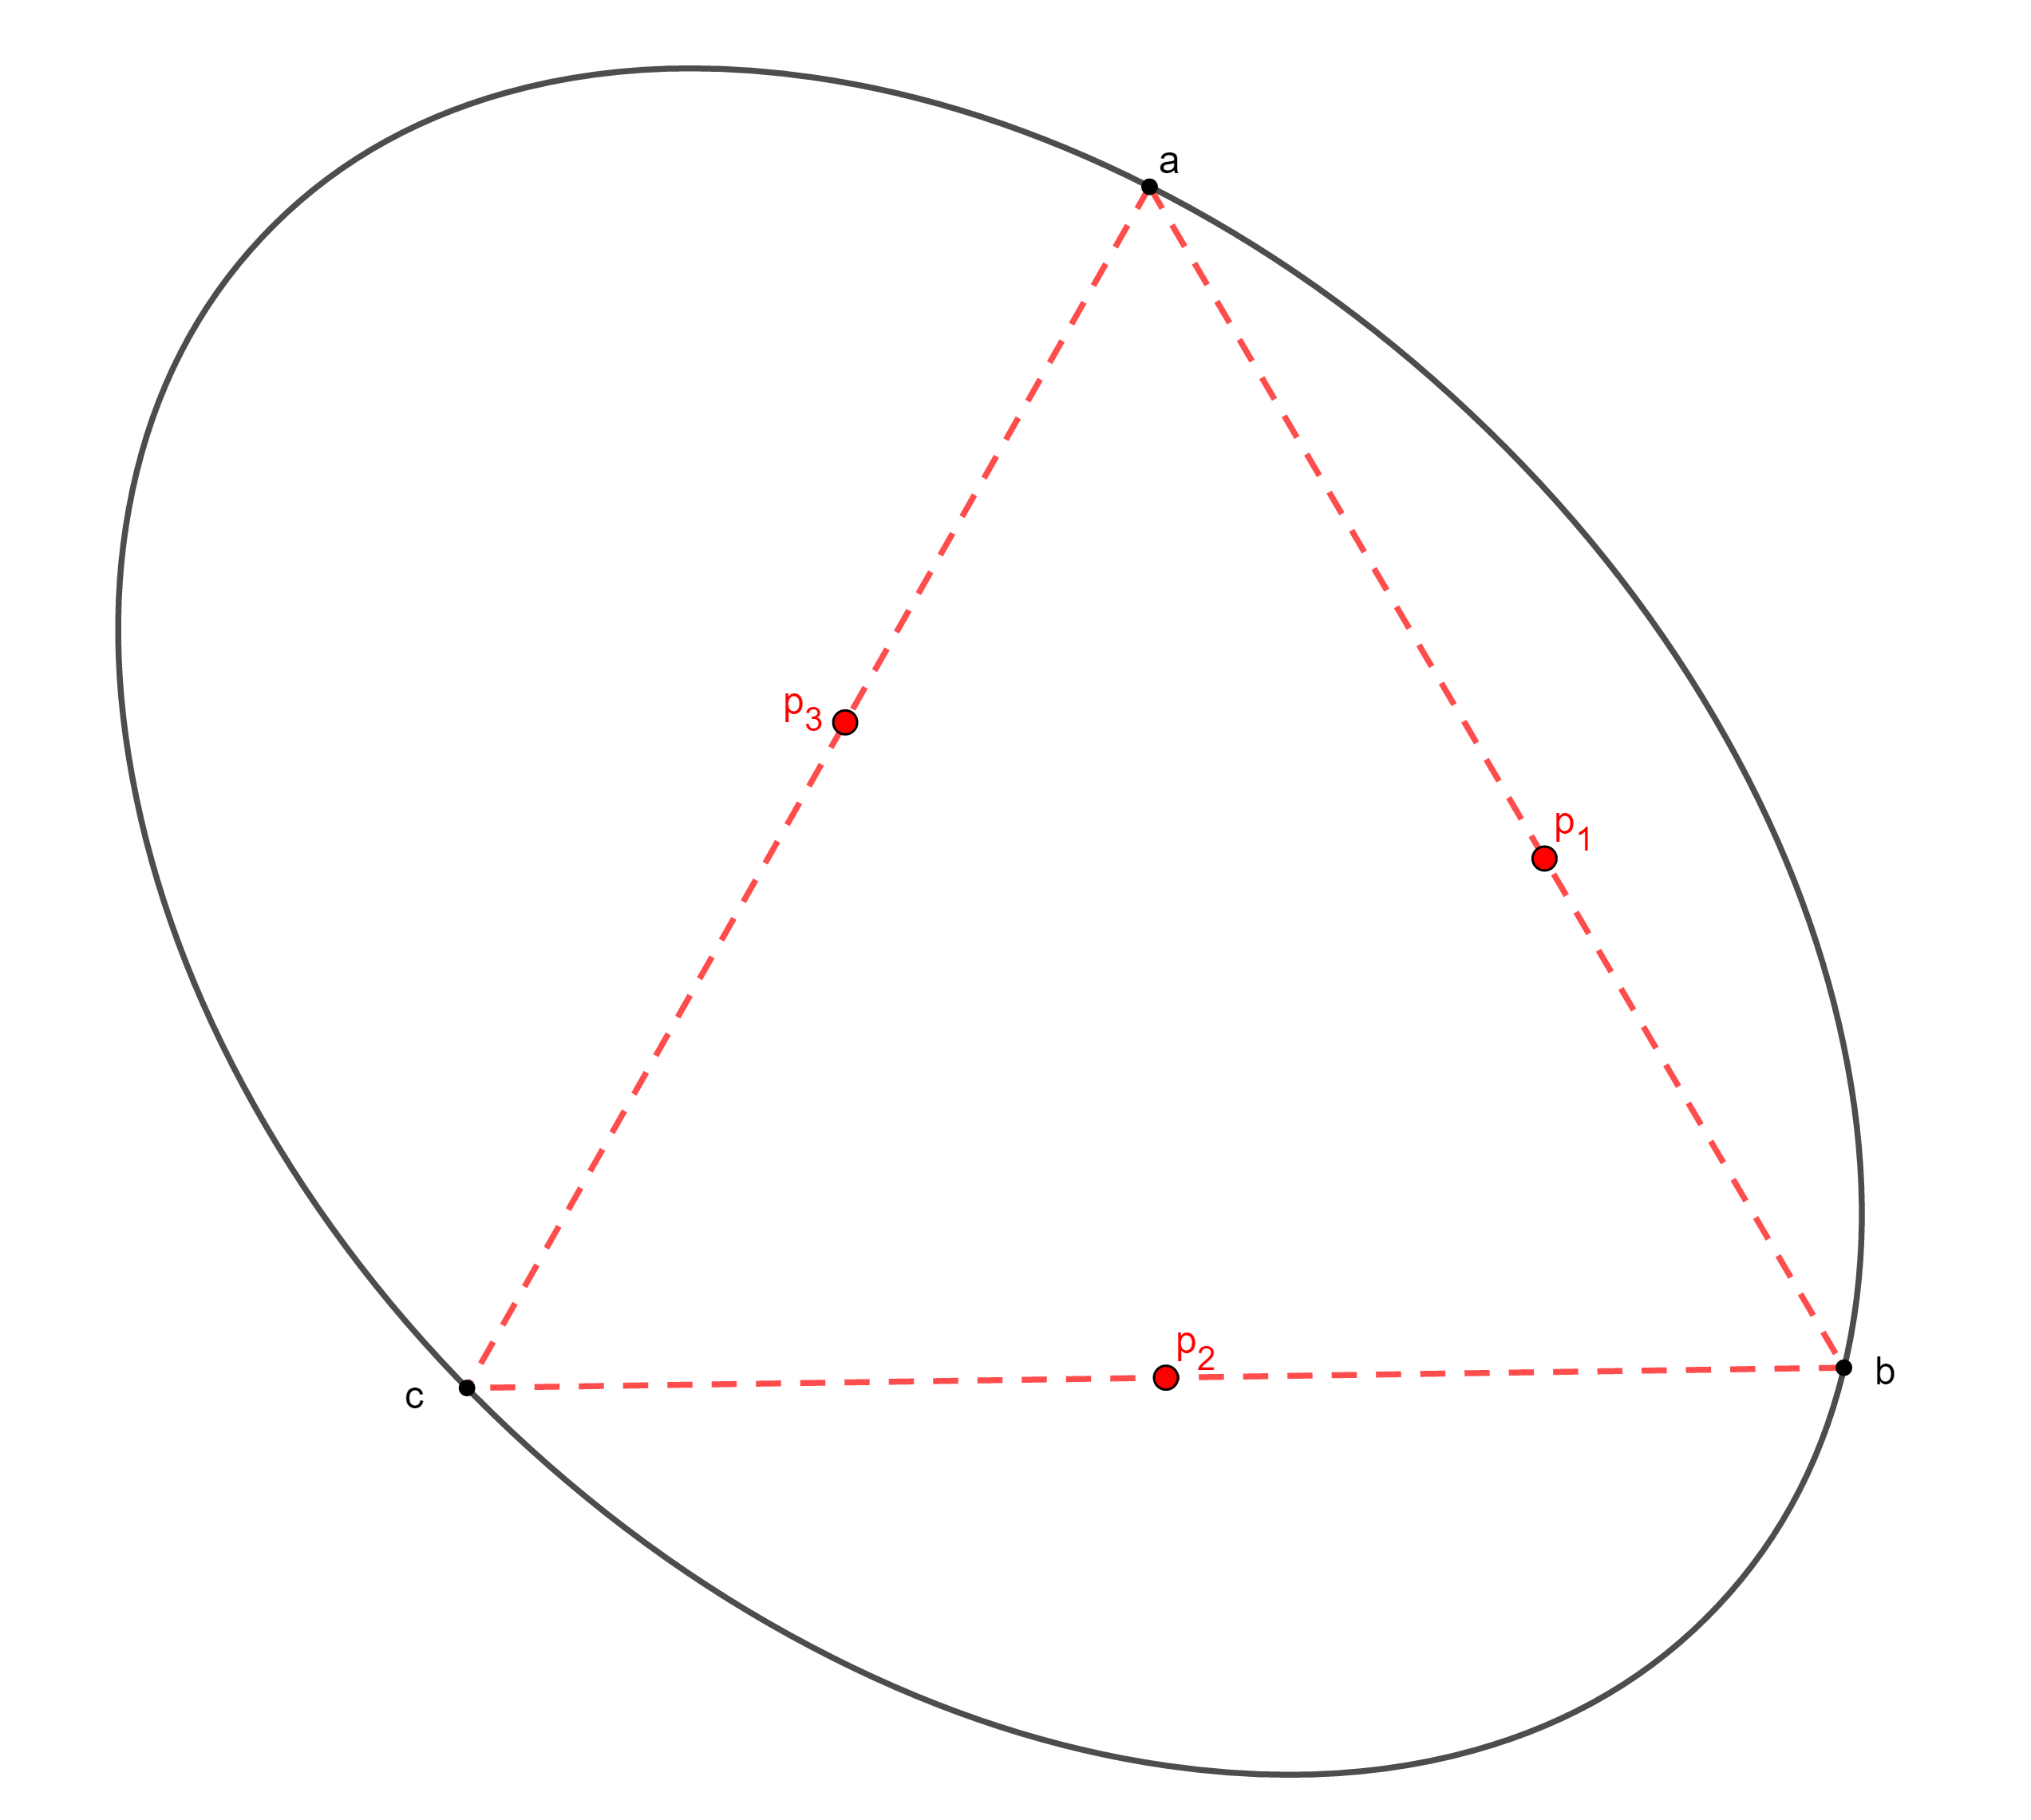
\includegraphics[width=0.8\linewidth]{pic15}}
			\end{minipage}
		\end{figure}
		\noindent
		Проведем преобразование как в одной из задач прошлого листочка -- представим наш треугольник в верхней полуплоскости с вершинами в точках $0,1,\infty$. Тогда можно заметить что $PS$ и $PR$ являются дугами орициклов. Докажем этот факт, рассмотрим картинку в верхней полуплоскости и заметим, что касательные к сторонам из точек $R,S$ совпадают с вертикальными сторонами, а следовательно центры окружностей (геодезических или орициклов), на которой лежат дуги $PS$ и $PR$, лежат на этих сторонах, а так как касательная проходящая через $P$ пересекает вертикальные стороны не в вершине, то $PS$ и $PR$ лежат на орициклах. Следовательно $\angle RPS$ это угол между орициклами, отмеченными на картинках красным. Тогда остается заметить, что эти орициклы касаются, а следовательно $\angle RPS = 0$.
		
		\subsection*{3}
		\noindent
		Заметим, что так как $\Gamma_i = e^{\frac{1}{2}a_i}$ то установив биекцию между треугольниками и тройками $(a_i,a_j,a_k)$ мы также установим биекцию между треугольниками и $(\Gamma_i, \Gamma_j,\Gamma_k)$, так как $\Gamma_i = e^{\frac{1}{2}a_i}$ задает биекцию между $(a_i,a_j,a_k)$ и $(\Gamma_i, \Gamma_j,\Gamma_k)$.
		\begin{figure}[h!]
			\center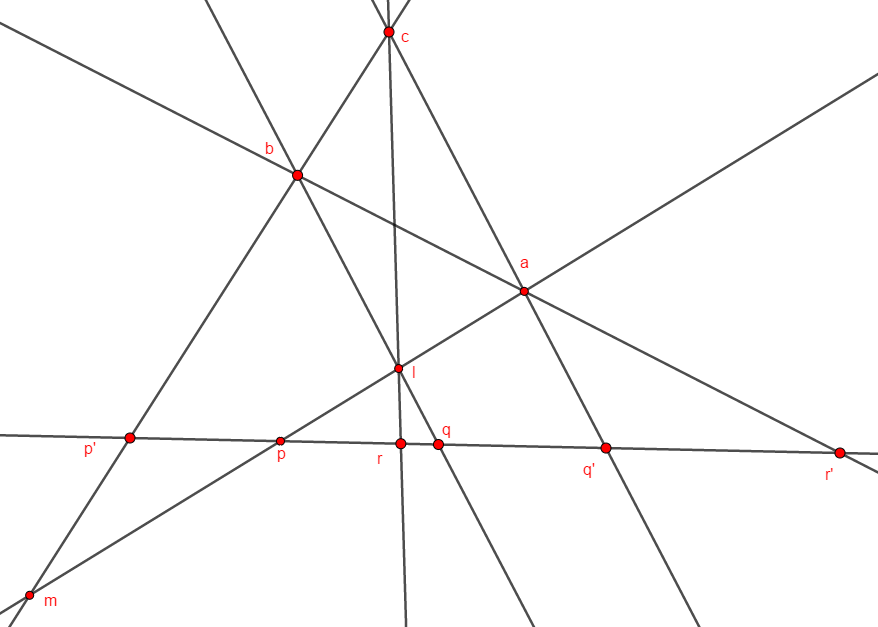
\includegraphics[width=0.5\linewidth]{pic9}
		\end{figure}\\
		Рассмотрим картинку, где красным отмечены орициклы $O_1, O_2, O_3$. Тогда заметим что участки геодезических отмеченные одним цветом(зеленым, оранжевым или фиолетовым) имеют равную длину и их длины мы можем вывести из $a_1, a_2, a_3$ (так как мы можем составить систему из 3 уравнений с 3 неизвестными). Также заметим, что по задаче 4 мы знаем $c_1, c_2, c_3$. Остается заметить, что из этого мы можем вывести длину цветных (зеленых, фиолетовых или рыжих) при любом размере красных орициклов, а следовательно и в случае нулевого радиуса, тогда мы получим длину 3 сторон, по которым однозначно восстанавливается идеальный треугольник.\\
		
		\subsection*{4}
		\begin{gather*}
			c_k = \frac{\Lambda_k}{\Lambda_i \Lambda_j} = \frac{e^{\frac{1}{2}a_{k}}}{e^{\frac{1}{2}a_{i}} e^{\frac{1}{2}a_{j}}} = e^{\frac{1}{2}a_{k}} \cdot e^{-\frac{1}{2}a_{i}} \cdot e^{-\frac{1}{2}a_{j}} = e^{\frac{1}{2}(a_{k} - a_{i} - a_{j})}
		\end{gather*}
		
		\subsection*{5*}
		\noindent
		Рассмотрим синий орицикл
		\begin{figure}[h]
			\center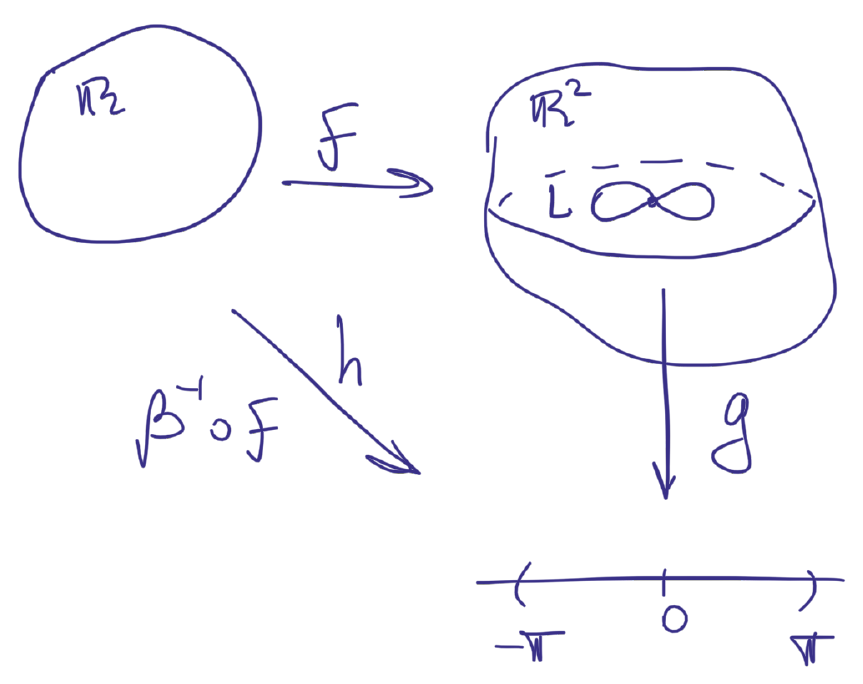
\includegraphics[width=0.65\linewidth]{pic10}
		\end{figure}\\
		Заметим что для дуги отмеченной красным выполнено:
		\begin{gather*}
			c_{13} = c_{12} + c_{23}\\
			\\
			\frac{\Lambda_{13}}{\Lambda_{14}\Lambda_{34}} = \frac{\Lambda_{12}}{\Lambda_{14}\Lambda_{24}} + \frac{\Lambda_{23}}{\Lambda_{24}\Lambda_{34}}
		\end{gather*}
		Домножим на $\Lambda_{14}\Lambda_{24}\Lambda_{34}$
		\begin{gather*}
			\Lambda_{13}\Lambda_{24} = \Lambda_{12}\Lambda_{34} + \Lambda_{23}\Lambda_{14}
		\end{gather*}
		
		\begin{comment}
		\subsection*{6*}
		\noindent
		Заметим что для всех треугольников данной фигуры должно быть выполнено неравенство треугольника 
		\begin{gather*}
		\end{gather*}
		\end{comment}	
\end{document}